% !TEX root = ./sub-main.tex
\documentclass[main.tex]{subfiles}

\begin{document}
    \subsection{Sources of funding costs}
        In the context of an OTC derivatives dealer, 
        \textcite{Ruiz2013FVA} mentions some of the most likely sources of funding costs as
        either asymmetry in collateral agreements or the payment liabilities due to the contract itself.
        Both of these sources will be discussed in the following sections.
        As will be concluded, funding costs contribute to the cost of trading under imperfect CSA agreements 
        and trading derivatives whose market risk cannot be perfectly replicated.

    \subsubsection{Funding costs from asymmetrical collateral agreements}
        If a perfect market risk hedge exists, funding costs can be viewed 
        as a component of the cost of trading derivatives that are not subject to a perfect CSA agreement.
        A perfect CSA agreement would require collateral to be posted continuously with no thresholds on the margin amounts,
        such that counterparty exposure is effectively eliminated.
        After entering financial contracts with counterparties,
        a derivatives dealer will often enter into the opposite trades
        with the sole purpose of hedging market risk.
        When the collateralization scheme with the counterparty is imperfect, 
        the collateral cash flows will most likely not match the collateral cash flows from the market risk hedges.
        This is often the case, as the dealer will likely hedge market risk in an exchange requiring full collateralization.
        Imbalance between the collateral schemes of the OTC deals and the market risk hedges
        is an origin of funding costs and the concern of this section.
        This source of funding costs is best introduced in its most extreme case, 
        where the dealer trades unsecured derivatives. 

        Consider the situation depicted in \cref{fig:funding-costs-unsecured-derivative}.
        The derivatives dealer is selling an unsecured OTC derivative to a counterparty,
        and the counterparty pays the upfront price.
        The particular type of derivative is not too important, 
        but picture a derivative that can leave the dealer both negatively and positively exposed to the counterparty, 
        e.g. an interest rate swap.
        In order to avoid the market risk of the investment, 
        the dealer will perform the opposite, perhaps synthetic, trade with an exchange,
        i.e. the dealer hedges its market risk to the counterparty.
        In this example, it is assumed that the upfront price of the derivative 
        matches exactly the upfront price of the market risk hedge.
        The exchange requires full collateralization;
        when the dealer has positive exposure to the counterparty, 
        it has negative exposure to the exchange and must post collateral. 
        When it has positive exposure to the counterparty it receives collateral.
        The collateral posted at the exchange is secured by the actual investment demanding the collateral;
        therefore, any collateral posted earns the OIS rate at the receiver, referred to as the rebate rate.
        The exchange could possibly charge a spread and pay a rebate rate less than the OIS rate,
        but for simplicity assume that this is not the case.
        Assume that the dealer has no excess cash on its balance sheet, 
        such that any collateral that needs to be posted to the exchange 
        must be borrowed from the dealer's funding institution,
        possibly its prime broker. 
        This funding is unsecured and the prime broker charges a spread, here denoted by S,
        more specifically the dealer pays the rate $\OIS/ + \text{S}$.

        The excess interest rate charged by the prime broker is exactly the source of the funding cost.
        If the dealer has positive exposure to the counterparty, collateral must be posted to the exchange.
        The dealer then earns \OIS/ from the posted collateral but pays $\OIS/ + \text{S}$ for funding;
        the difference, S, drives the funding cost.
        Alternatively, the exchange posts collateral to the dealer, which the dealer pays \OIS/ for.
        If rehypothecation is allowed, the dealer can retire debt and save the funding spread.
        In this case, S drives the funding benefit.

        \begin{figure}
            \centering
            \resizebox{\textwidth}{!}{%
            \begin{tikzpicture}
                % !TEX root = ./test-graphics.tex

\tikzmath{
    \arrowyoffset = 7;
    \arrowcenteryoffset = 7;
    \toparrowyoffset = \arrowcenteryoffset + \arrowyoffset;
    \bottomarrowyoffset = \arrowcenteryoffset - \arrowyoffset;
    \arrowtoboxpadding = 5;
}
\coordinate (center) at (0,0);
\node (dealer) at (center) [
    draw,
    fill=white!80!gray,
    very thick,
    minimum width=3cm,
    minimum height=2cm,
    align=center,
    rounded corners=.50cm,
] {Derivatives\\dealer};

\node (counterparty) at ($(dealer.west) + (-5, 0)$) [
    draw,
    very thick,
    minimum width=3cm,
    minimum height=2cm
] {Counterparty};

\node (exchange) at ($(dealer.east) + (5, 0)$) [
    draw,
    dashed,
    very thick,
    minimum width=3cm,
    minimum height=2cm,
] {Exchange};

\node (funding) at ($(dealer.south) + (0, -4)$) [
    draw,
    very thick,
    minimum width=3cm,
    minimum height=2cm,
] {Prime broker};

% Dealer - Counterparty relations
\draw[->, thick] 
    ([yshift=\bottomarrowyoffset pt, xshift=-\arrowtoboxpadding pt]dealer.south west) -- 
    ([yshift=\bottomarrowyoffset pt, xshift= \arrowtoboxpadding pt]counterparty.south east)
    node[near start, fill=white, inner sep=0pt] {
        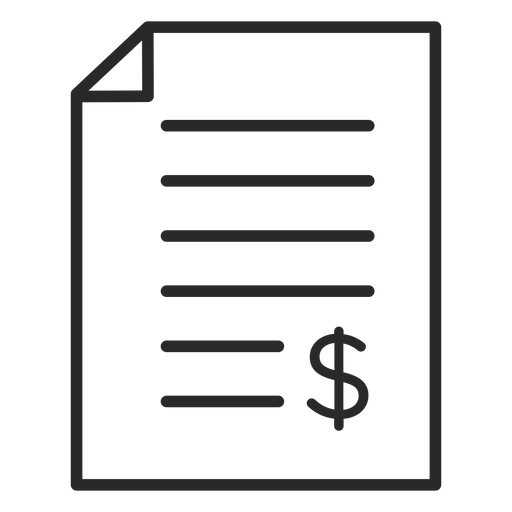
\includegraphics[width=0.60cm]{\graphicsfolder/source-of-funding-costs/contract}
    };
\draw[<-, thick] 
    ([yshift=\toparrowyoffset pt, xshift=-\arrowtoboxpadding pt]dealer.south west) -- 
    ([yshift=\toparrowyoffset pt, xshift= \arrowtoboxpadding pt]counterparty.south east)
    node[near end, fill=white, inner sep=2pt] {
        \$\$\$
    };

% Dealer - Exchange relations
\draw[<-, thick] 
    ([yshift=\bottomarrowyoffset, xshift= \arrowtoboxpadding pt]dealer.south east) -- 
    ([yshift=\bottomarrowyoffset, xshift=-\arrowtoboxpadding pt]exchange.south west)
    node[near end, fill=white, inner sep=0pt] {
        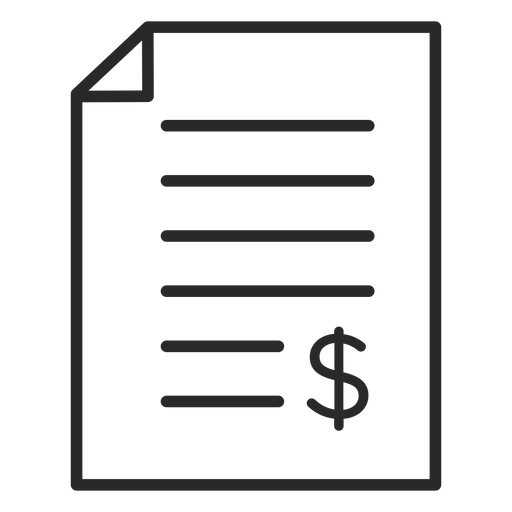
\includegraphics[width=0.60cm]{\graphicsfolder/source-of-funding-costs/contract}
    };
\draw[->, thick] 
    ([yshift=\toparrowyoffset, xshift= \arrowtoboxpadding pt]dealer.south east) -- 
    ([yshift=\toparrowyoffset, xshift=-\arrowtoboxpadding pt]exchange.south west)
    node[near start, fill=white, inner sep=2pt] {
        \$\$\$
    };

\draw[<->, thick, draw=blue] 
    ([yshift=-\bottomarrowyoffset, xshift= \arrowtoboxpadding pt]dealer.north east) -- 
    ([yshift=-\bottomarrowyoffset, xshift=-\arrowtoboxpadding pt]exchange.north west)
    node [pos=0.4, fill=white, inner sep=0pt] {
        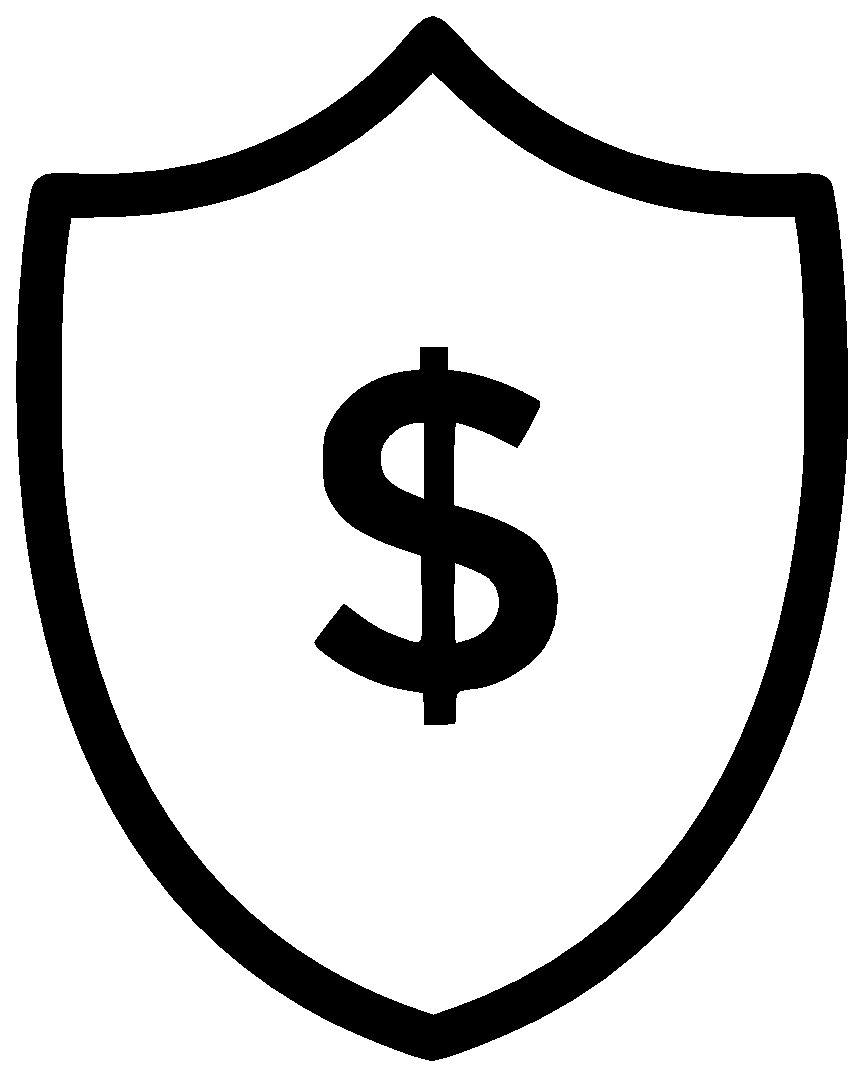
\includegraphics[width=0.65cm]{\graphicsfolder/source-of-funding-costs/collateral}
    };
\draw[<->, thick, draw=red] 
    ([yshift=-\toparrowyoffset, xshift= \arrowtoboxpadding pt]dealer.north east) -- 
    ([yshift=-\toparrowyoffset, xshift=-\arrowtoboxpadding pt]exchange.north west)
    node [pos=0.6, fill=white, inner xsep=2pt, inner ysep=0] {
        OIS
    };

% Dealer - Funding relations
\draw[<->, thick, draw=blue]
    ([xshift=-\arrowyoffset, yshift=-\arrowtoboxpadding]dealer.south) --
    ([xshift=-\arrowyoffset, yshift= \arrowtoboxpadding]funding.north)
    node[midway, fill=white, inner xsep=2pt, inner ysep=0, align=center, rotate=90] {
        Funding
    };
\draw[<->, thick, draw=red]
    ([xshift=\arrowyoffset, yshift=-\arrowtoboxpadding]dealer.south) --
    ([xshift=\arrowyoffset, yshift= \arrowtoboxpadding]funding.north)
    node[midway, fill=white, inner xsep=2pt, inner ysep=0, align=center, rotate=90] {
        OIS + S
    };
            \end{tikzpicture}        
            }   
            \caption{Illustration of funding costs from an unsecured OTC derivative.}
            \label{fig:funding-costs-unsecured-derivative}
        \end{figure}

        As mentioned, trading unsecured derivatives is the most extreme case,
        since any collateral call will lead to a funding surplus or deficit and therefore a funding benefit or cost.
        The funding cost can be reduced if the dealer has in place 
        a CSA agreement allowing rehypothecation with the counterparty.
        This would allow collateral to flow from the exchange to the counterparty or the opposite direction, 
        and collateral postings from one party could therefore, partly or fully, 
        cover collateral needs from the other party.

        Consider the example illustrated in \cref{fig:funding-costs-secured-derivative}.
        Again, the dealer sells a derivative to its counterparty,
        but in this case the two parties are trading under a CSA agreement, 
        such that the trade is secured by collateralization.
        The posting of collateral by the counterparty reduces the credit risk of the dealer,
        but the dealer still faces the market risk from the derivative;
        so, again, it creates a market risk hedge at the exchange.
        Assume a perfect hedge, such that any market risk exposure to the counterparty 
        is exactly offset by the opposite exposure to the exchange.
        Whenever there is a collateral call from the dealer to the counterparty,
        the dealer can expect a call for collateral from the exchange.
        Since rehypothecation is allowed,
        the collateral posted by the counterparty can be passed onto the exchange.
        To a certain extent, this reduces the dealer's need for borrowing unsecured funds from the prime broker
        and ultimately reduces the funding costs of the dealer.
        However, funding costs are possibly still present;
        the collateral agreement with the counterparty is likely weaker than that with the exchange. 
        This is depicted in \cref{fig:funding-costs-secured-derivative} 
        by the shield on the counterparty side being smaller than the shield on the exchange side.
        The asymmetry has the implications that 
        collateral posted by the counterparty might only partly cover collateral calls from the exchange 
        and collateral posted by the exchange will more than cover collateral calls from the counterparty.
        The former is a source of funding costs and the latter a source of funding benefit.

        The differences between the CSA agreements, leading to the situation described above, could vary. 
        To mention a few, the CSA agreement with the counterparty might have higher exposure thresholds, 
        higher minimum transfer amounts, or lower frequency of margin calls.
        All of these differences lead the collateral cash flows to and from the exchange 
        to be at least as high as the cash flows to and from the counterparty. 
        In case the two collateral agreements are identical, the funding cost will be eliminated, 
        since the collateral received from the counterparty will completely suffice as collateral posted to the exchange.
        
        \begin{figure}
            \centering
            \resizebox{\textwidth}{!}{%
            \begin{tikzpicture}
                % !TEX root = ./test-graphics.tex

% !TEX root = ./test-graphics.tex

\tikzmath{
    \arrowyoffset = 7;
    \arrowcenteryoffset = 7;
    \toparrowyoffset = \arrowcenteryoffset + \arrowyoffset;
    \bottomarrowyoffset = \arrowcenteryoffset - \arrowyoffset;
    \arrowtoboxpadding = 5;
}
\coordinate (center) at (0,0);
\node (dealer) at (center) [
    draw,
    fill=white!80!gray,
    very thick,
    minimum width=3cm,
    minimum height=2cm,
    align=center,
    rounded corners=.50cm,
] {Derivatives\\dealer};

\node (counterparty) at ($(dealer.west) + (-5, 0)$) [
    draw,
    very thick,
    minimum width=3cm,
    minimum height=2cm
] {Counterparty};

\node (exchange) at ($(dealer.east) + (5, 0)$) [
    draw,
    dashed,
    very thick,
    minimum width=3cm,
    minimum height=2cm,
] {Exchange};

\node (funding) at ($(dealer.south) + (0, -4)$) [
    draw,
    very thick,
    minimum width=3cm,
    minimum height=2cm,
] {Prime broker};

% Dealer - Counterparty relations
\draw[->, thick] 
    ([yshift=\bottomarrowyoffset pt, xshift=-\arrowtoboxpadding pt]dealer.south west) -- 
    ([yshift=\bottomarrowyoffset pt, xshift= \arrowtoboxpadding pt]counterparty.south east)
    node[near start, fill=white, inner sep=0pt] {
        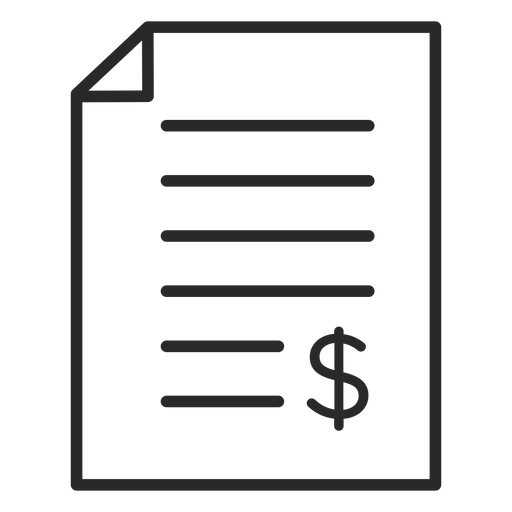
\includegraphics[width=0.60cm]{\graphicsfolder/source-of-funding-costs/contract}
    };
\draw[<-, thick] 
    ([yshift=\toparrowyoffset pt, xshift=-\arrowtoboxpadding pt]dealer.south west) -- 
    ([yshift=\toparrowyoffset pt, xshift= \arrowtoboxpadding pt]counterparty.south east)
    node[near end, fill=white, inner sep=2pt] {
        \$\$\$
    };

% Dealer - Exchange relations
\draw[<-, thick] 
    ([yshift=\bottomarrowyoffset, xshift= \arrowtoboxpadding pt]dealer.south east) -- 
    ([yshift=\bottomarrowyoffset, xshift=-\arrowtoboxpadding pt]exchange.south west)
    node[near end, fill=white, inner sep=0pt] {
        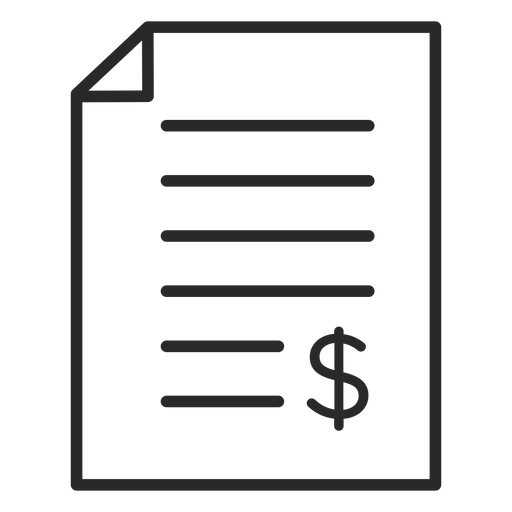
\includegraphics[width=0.60cm]{\graphicsfolder/source-of-funding-costs/contract}
    };
\draw[->, thick] 
    ([yshift=\toparrowyoffset, xshift= \arrowtoboxpadding pt]dealer.south east) -- 
    ([yshift=\toparrowyoffset, xshift=-\arrowtoboxpadding pt]exchange.south west)
    node[near start, fill=white, inner sep=2pt] {
        \$\$\$
    };

\draw[<->, thick, draw=blue] 
    ([yshift=-\bottomarrowyoffset, xshift= \arrowtoboxpadding pt]dealer.north east) -- 
    ([yshift=-\bottomarrowyoffset, xshift=-\arrowtoboxpadding pt]exchange.north west)
    node [pos=0.4, fill=white, inner sep=0pt] {
        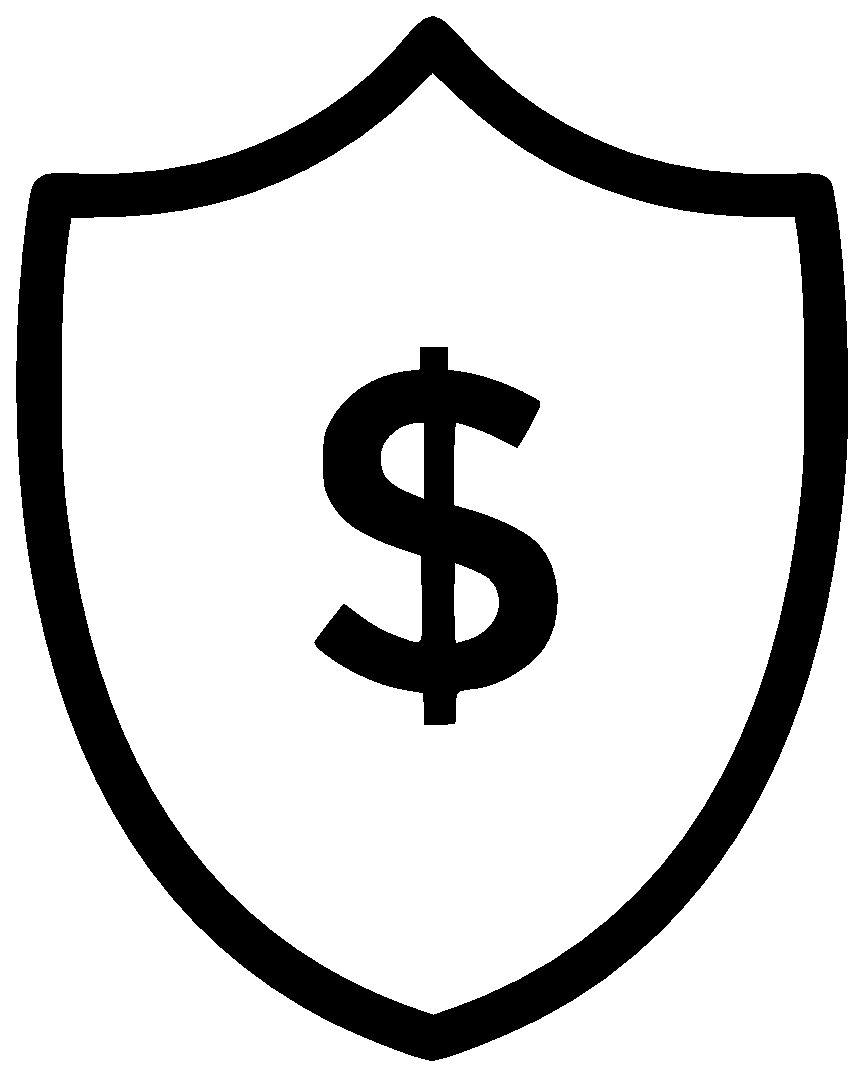
\includegraphics[width=0.65cm]{\graphicsfolder/source-of-funding-costs/collateral}
    };
\draw[<->, thick, draw=red] 
    ([yshift=-\toparrowyoffset, xshift= \arrowtoboxpadding pt]dealer.north east) -- 
    ([yshift=-\toparrowyoffset, xshift=-\arrowtoboxpadding pt]exchange.north west)
    node [pos=0.6, fill=white, inner xsep=2pt, inner ysep=0] {
        OIS
    };

% Dealer - Funding relations
\draw[<->, thick, draw=blue]
    ([xshift=-\arrowyoffset, yshift=-\arrowtoboxpadding]dealer.south) --
    ([xshift=-\arrowyoffset, yshift= \arrowtoboxpadding]funding.north)
    node[midway, fill=white, inner xsep=2pt, inner ysep=0, align=center, rotate=90] {
        Funding
    };
\draw[<->, thick, draw=red]
    ([xshift=\arrowyoffset, yshift=-\arrowtoboxpadding]dealer.south) --
    ([xshift=\arrowyoffset, yshift= \arrowtoboxpadding]funding.north)
    node[midway, fill=white, inner xsep=2pt, inner ysep=0, align=center, rotate=90] {
        OIS + S
    };

\draw[<->, thick, draw=fundingcolor] 
    ([yshift=-\bottomarrowyoffset, xshift=-\arrowtoboxpadding pt]dealer.north west) -- 
    ([yshift=-\bottomarrowyoffset, xshift= \arrowtoboxpadding pt]counterparty.north east)
    node (collateral) [pos=0.6, fill=white, inner sep=0pt] {
        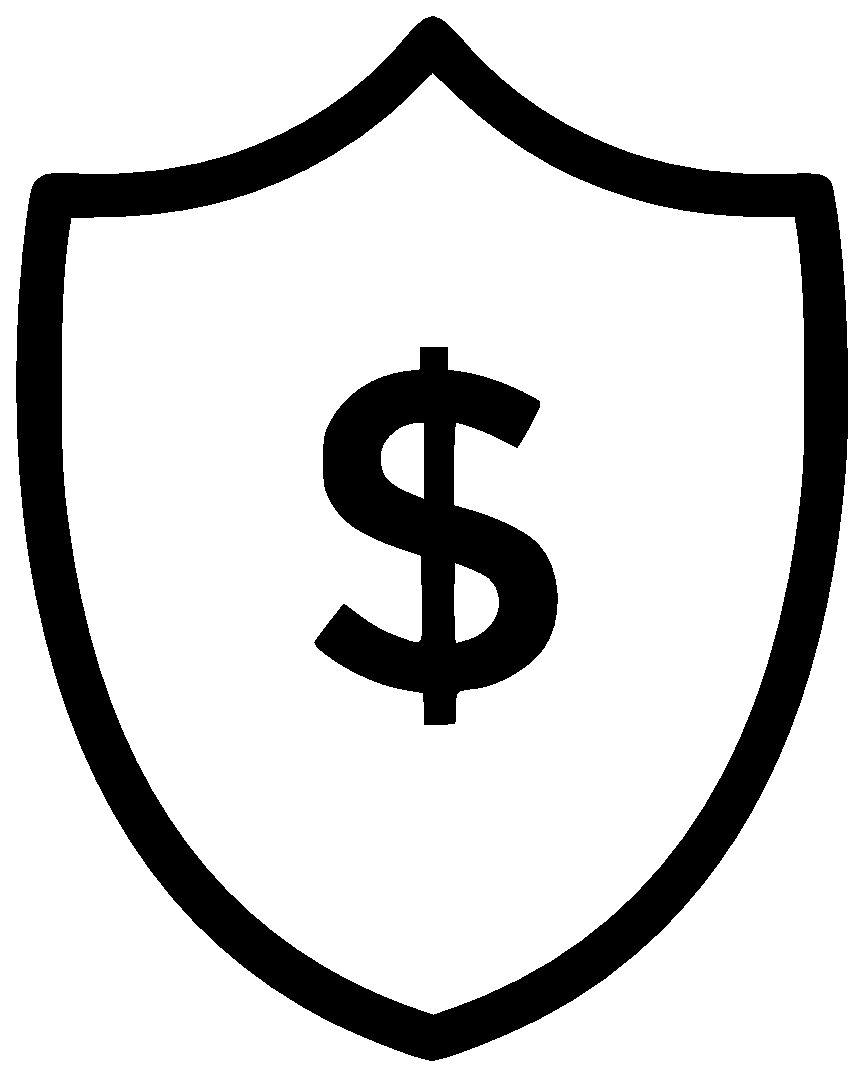
\includegraphics[width=0.40cm]{\graphicsfolder/source-of-funding-costs/collateral}
    };


\draw[<->, thick, draw=ratecolor] 
    ([yshift=-\toparrowyoffset, xshift=-\arrowtoboxpadding pt]dealer.north west) -- 
    ([yshift=-\toparrowyoffset, xshift= \arrowtoboxpadding pt]counterparty.north east)
    node [pos=0.4, fill=white, inner xsep=2pt, inner ysep=0] {
        OIS
    };
            \end{tikzpicture}        
            }   
            \caption{Illustration of funding costs from an secured OTC derivative.}
            \label{fig:funding-costs-secured-derivative}
        \end{figure}

        These examples should display how a derivatives dealer might face funding costs,
        when the lack of perfect symmetry in collateral needs calls for unsecured funding.
        It might be argued that the funding costs could be eliminated by trading derivatives,
        whose replication can be operated by repurchase agreements. 
        Seemingly, buying the hedging strategy at repo should eliminate the need for unsecured financing
        and thus the funding costs. 
        However, even when repo market exists, hedging might require unsecured funding,
        which can be shown with an example by \textcite{Castagna2012FVA}.
        Consider a dealer buying a european call option, with the intention to hedge the market risk.
        To create the hedging strategy the dealer must short an amount of the underlying asset corresponding to the option Delta of the call option.
        If the underlying asset can be sold at repo the dealer will receive the repo rate.
        However, to pay the premium for the call option the dealer must borrow unsecured funds from its funding institution,
        paying again the funding spread. 

        For financial institutions, funding costs, as the aforementioned, justifies an adjustment 
        to the derivatives' price corresponding to the funding cost the derivatives introduce if they are obtained.
        This justification is however refused by \textcite{HullWhite2012FVA}.
        They state that, since a hedge consists of buying and selling assets for their market prices,
        performing a hedge is an investment with zero net present value.
        Exchanging money for assets of identical value,
        is simply moving value around and these operations should not influence valuations. 

        In any case,
        the funding spread could very well be part of the hedging strategy which makes it undeniable for dealers when performing valuation of the initial investments.

        Another argument proposed by \textcite{HullWhite2012FVA} is the fact that dealers buy Treasury instruments and other low-yielding assets returning less than the dealers' average funding cost.
        They do this without applying an FVA and the implication of the argument is that there is an inconsistency in dealer practice,
        as the low-yielding instruments would be unprofitable if an FVA was made.
        The previous discussion however nests an explanation for this dealer behaviour.
        For Treasury instruments and the like,
        very developed repo markets exists such that the purchase of these instruments can be financed with secured funding.
        Consequently the funding cost of buying these instruments is likely much lower than the dealers' average funding cost,
        which partly explains why dealers willingly buy them.
        As shown by the example of the OTC derivatives dealer, 
        the lack of a repo market for derivatives is exactly the reason why funding costs appear in the first place.
        In fact \textcite[Section~9.4.1]{Green2015XVA}, 
        using the \footcite{BurgardKjaer2013Funding} Semi-Replication model,
        shows that the existence of a repo market would eliminate the need for an \FVA/ on derivatives. 
        
    \subsubsection{Funding costs from derivatives cash flows}
        The fact that the dealer does not have access to risk-free funding
        can imply further contributions to the funding costs, besides that from collateral financing.
        First, note that cash flows arising from a derivative must also be funded at a non-risk-free rate
        and that these cash flows can be used for netting other cash flows in the dealer's portfolio.
        The second point implies that with the existence of a perfect replication,
        the cash flows from a derivative can be completely offset by the hedging strategy,
        such that no additional funding is required and no funding costs are generated.

        In reality, replications of OTC derivatives are most often imperfect,
        such that there is no one-to-one correspondence in cash flows between the derivative and the hedge.
        Of course, the dealer might not even try to hedge a derivative directly,
        but rather let a netting set of cash flows offset each other. 
        The principle is the same whether the derivative cash flows are offset by an imperfect hedge
        or another different derivative;
        both are again sources of funding cost, which can be illustrated by the following examples.

        The treatment of derivative cash flows from a funding cost perspective 
        depends on the type of cash flow and the reason why it occurs,
        as not all entail funding costs for the same reason.

        Consider a firm buying a simple option, without the intention to hedge its market risk.
        Buying the option requires paying an upfront price to the counterparty,
        which would seemingly require financing;
        however, this is only a source of funding costs 
        if the firm and the counterparty do not have a CSA agreement in place.
        If both the firm and the counterparty are financial institutions, 
        they will most likely maintain a CSA agreement
        such that any upfront price paid will immediately be met by a collateral posting in the opposite direction.
        Hence, the funding need for the upfront price will be satisfied and the funding costs eliminated.
        If no CSA exists and no collateral is posted, the upfront will still create funding costs,
        while selling the option instead will decrease the funding needs and create a funding benefit.
        This is not to say that a CSA agreement will eliminate funding costs completely. 
        Hedging cash flows might also generate funding needs or surpluses, 
        e.g. if a dealer must apply leverage to properly hedge a positions 
        and pay the higher rates of leverage due to financing spreads.

        Another source of funding costs materializes in the next example when the dealer applies an imperfect hedge.
        The dealer have entered into a 10 year OTC swap with semi-annual payments, 
        but for the replication the dealer is only able to obtain a 10 year swap with quarterly payments.
        As a result, the dealer will have a cash flow from the hedge every three months
        that does not correspond to the cash flow from the OTC derivative. 
        Both of these are examples of funding costs essentially stemming from the lack of perfect hedging.

        Having established some possible sources of funding costs, 
        the discussion can move on to the debate about whether accounting for these is appropriate for derivatives pricing.

\end{document}
        